\documentclass{article}

\usepackage[utf8]{inputenc}
\usepackage[T1]{fontenc}
\usepackage[francais]{babel}
\usepackage{titling}
\setlength{\droptitle}{-3cm}
\usepackage{graphicx}
\usepackage{underscore}
\usepackage{hyperref} 

\title{Les données et leur exploration}
\author{CAROT Axel, ARISOY Ivan Can, \\ DARDE Guilhem, NDJINGA NDJINGA Anta Claude}
\date{\today}

\begin{document}
\maketitle

\section{Collecte des données}
Les documents pertinents concernant la sécurité alimentaire ont été récoltés puis triés grâce à une série d'étapes de prétraitement, différentes pour chaque type de média. 

\subsection{Acquisition de données}
Pour les articles de presse, la première étape est l'acquisition des articles sur le Web (web-scraping des articles sur les sites web des principaux médias de la région). Pour obtenir des documents à partir de vidéos, l'acquisition a été réalisée grâce aux transcriptions générées automatiquement par YouTube. Cette tâche s'appuie sur une bibliothèque Python exploitant l'API de Transcription/Sous-titres de YouTube. Les documents obtenus fournissent une version textuelle des discours dans les vidéos.

\subsection{Enrichissement des données}
Nous avons décidé d'enrichir les données avec des données radio transcrites. Pour cela, nous avons en premier lieu sélectionné les radios locales abordant la thématique. \\

Une fois que les stations radio traitant de cette thématique sont identifiées, nous utiliserons une méthode de web scraping et la bibliothèque Python BeautifulSoup. Nous procéderons à une transcription de ces données audio en texte à l'aide de la bibliothèque SpeechRecognition. \\

Cet enrichissement des données n'aura en termes de coût que le temps de mise en pratique de ces techniques et n'engendrera pas de coût financier. 

\subsection{Traitement de texte, text processing}
Une fois les documents obtenus, des étapes de prétraitement sont effectuées. Les mots sont extraits du texte (tokenisation). Ces mots sont remplacés par des lemmes (lemmatisation). Les mots vides qui n'ont pas de signification sont supprimés. Pour finir, les documents sont représentés de manière vectorielle (vectorisation avec la bibliothèque Python Punctuator, entraînée sur Wikipedia en français). 

\begin{figure}[h]
    \centering
    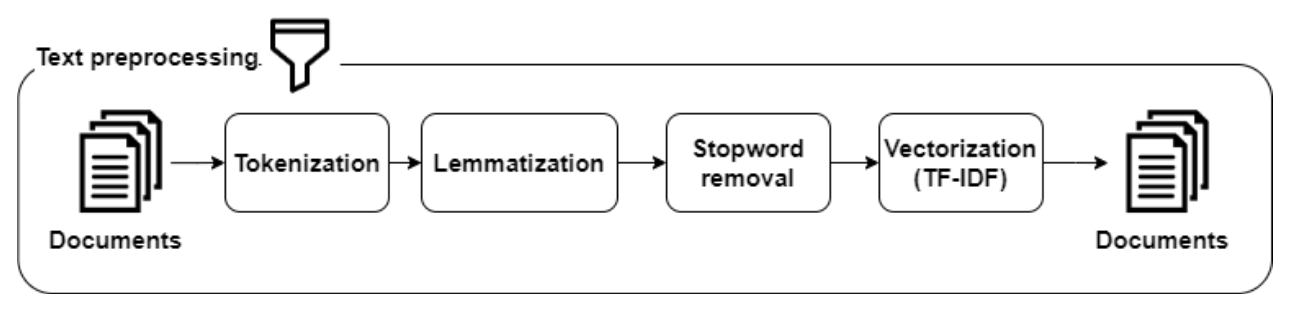
\includegraphics[width=0.8\textwidth]{text_process.png}
    \caption{Nombre de mots-clés par catégorie}
    \label{fig:keops_fraiberger}
\end{figure}

\section{Les données}
\subsection{Le corpus}
Nous disposons d'un corpus d'articles dans un fichier "\textbf{corpus_BF.xlsx}" en format Excel avec un mélange de types de données (numérique, texte). \\

Caractéristiques du fichier :
\begin{itemize}
    \item Nombre total d'entrées : 22,856
    \item Nombre total de colonnes : 8 \\
\end{itemize}

Dictionnaire des variables :
\begin{itemize}
    \item ANNEE (int64) : Année de l'article.
    \item SIM_W2V (float64) : Mesure de similarité obtenue à l'aide de Word2Vec.
    \item NEG (float64) : Indicateur de négativité mis en place par les commanditaires.
    \item VOC_SA (object) et VOC_CR (object) : Mots-clés similaires avec le lexique.
    \item REGION_CITE (object) : Région ou lieu cité dans l'article.
    \item NB_MOTS (int64) : Nombre de mots dans l'article.
    \item TXT (object) : Texte de l'article. \\
\end{itemize}

La population concernée représente les articles et transcriptions YouTube en Afrique de l'Ouest sur le thème de l'insécurité alimentaire. Les unités statistiques sont chaque article et transcription. 

\subsection{Les lexiques}
Le fichier "\textbf{expert.xlsx}" est un lexique français élaboré dans le cadre de la thèse de doctorat de Hugo Deléglise. Il se compose de 3 ensembles de mots-clés sur la sécurité alimentaire et les crises adaptés au contexte du Burkina Faso sur la période 2009-2018 créés par plusieurs experts en sécurité alimentaire : un lexique général sur la sécurité alimentaire composé de 21 expressions (LEXG) ; un lexique détaillé sur la sécurité alimentaire composé de 84 expressions (LEXA) ; un lexique détaillé sur les crises composé de 83 expressions (LEXC) (30-08-2021). \\

Le fichier "\textbf{fraiberger.xlsx}" est un lexique français élaboré dans le contexte d'un projet de partenariat de recherche et d'innovation UE-UA pour la sécurité alimentaire et l'agriculture durable. Le lexique est structuré en deux colonnes : 331 mots-clés (colonne 1) associés à 12 concepts (colonne 2). \\

Le fichier "\textbf{KEOPS.xlsx}" fait partie du résultat d'une étude récente sur le suivi de la sécurité alimentaire basée sur les nouvelles. Des mots-clés liés aux facteurs de risque de sécurité alimentaire ont été extraits d'un large corpus de nouvelles en ligne en anglais, en utilisant des méthodes basées sur des modèles et des méthodes d'incorporation de mots, et filtrés statistiquement pour obtenir 164 mots-clés finaux. Ils ont été manuellement regroupés en 12 grappes sémantiques. Ils ont été traduits en français en utilisant le ChatGPT en ligne et en vérifiant manuellement la cohérence.

\section{Analyses descriptives}
\begin{figure}[h]
    \centering
    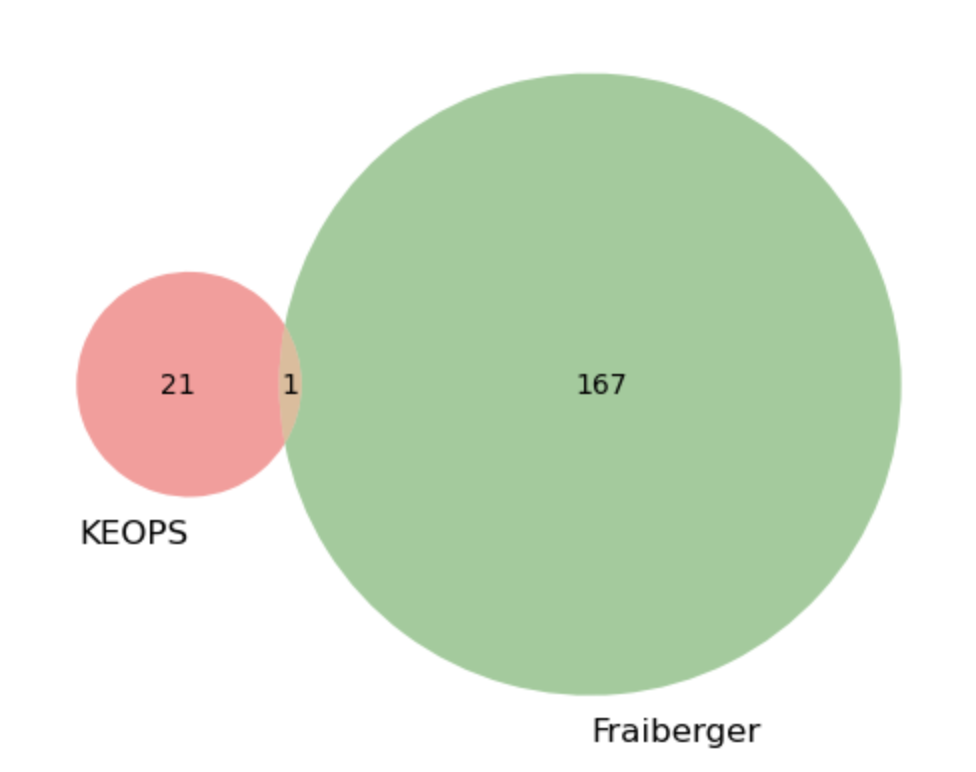
\includegraphics[width=0.4\textwidth]{keops_fraiberger.png}
    \caption{Diagramme de Venn illustrant les chevauchements entre les lexiques keops et fraiberger }
    \label{fig:keops_fraiberger}
\end{figure}

\begin{figure}[h]
    \centering
    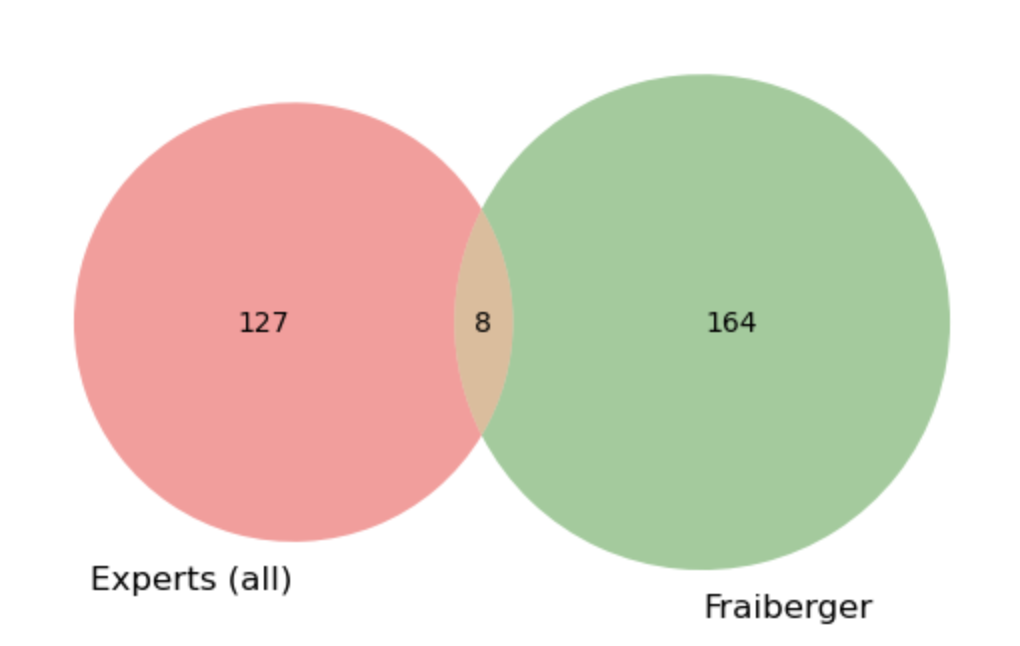
\includegraphics[width=0.4\textwidth]{expert_fraiberger.png}
    \caption{Diagramme de Venn illustrant les chevauchements entre les lexiques expert et fraiberger}
    \label{fig:expert_fraiberger}
\end{figure}
\vspace{2cm}
Dans le premier diagramme, l'intersection où les deux cercles se chevauchent, représente 1 mot-clé qui est commun aux deux lexiques. Dans le second diagramme, l'intersection où les deux cercles se chevauchent, représente 8 mot-clé qui est commun aux deux lexiques. \\

Dans les deux cas, le nombre de mots-clés exclusifs à chaque ensemble est notablement plus élevé que ceux partagés, indiquant une diversité d'approches et de priorités dans la conceptualisation des enjeux de sécurité alimentaire et de crises.
\vspace{0.5cm}

\begin{figure}[h]
    \centering
    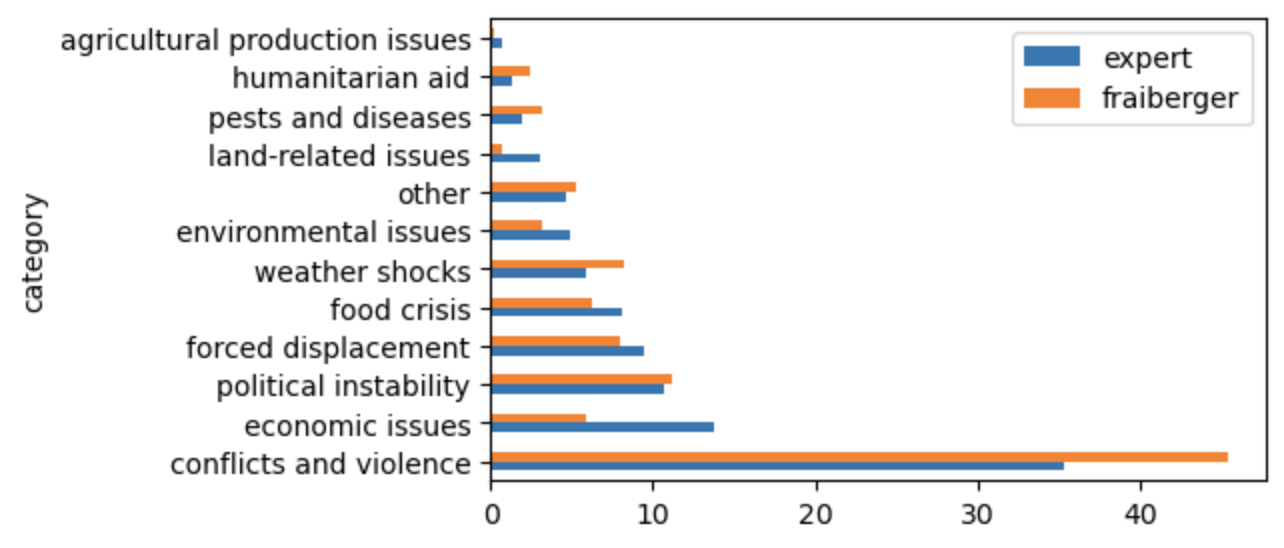
\includegraphics[width=0.8\textwidth]{freq_cat.png}
    \caption{Comparaison du nombre de mots-clés attribués à diverses catégories pour les lexiques expert et fraiberger}
    \label{fig:freq_cat}
\end{figure}
\vspace{0.5cm}

Ce graphique en barres horizontales compare le nombre de mots-clés attribués à diverses catégories par le lexique expert et par le lexique Fraiberger. La catégorie "conflicts and violence" possède le plus grand nombre de mots-clés attribués à la fois par les experts et Fraiberger, ce qui suggère une importance considérable accordée aux conflits et à la violence dans le contexte de la sécurité alimentaire. "Economic issues" et "political instability" sont également des catégories avec un nombre relativement élevé de mots-clés, indiquant que les problèmes économiques et la stabilité politique sont considérés comme des facteurs clés influençant la sécurité alimentaire.

\begin{figure}[h]
    \centering
    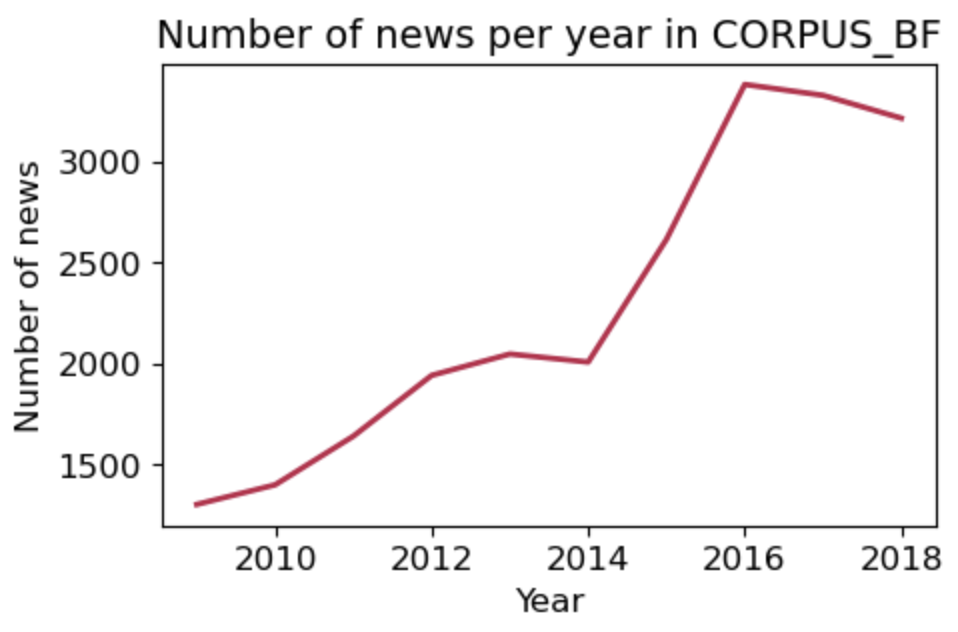
\includegraphics[width=0.8\textwidth]{nbr_articles_an.png}
    \caption{Tendance croissante du nombre de nouvelles par an dans le corpus CORPUS_BF}
    \label{fig:nbr_articles_an}
\end{figure}
\vspace{6cm}

Ce graphique indique une tendance croissante du nombre de nouvelles par an dans le corpus de données CORPUS_BF de 2010 à 2016. Une légère diminution à partir de 2016.

\end{document}
